\documentclass[graybox,envcountchap,sectrefs]{svmono}

\usepackage{type1cm}         

\usepackage{makeidx}         
\usepackage{graphicx}        
                            
\usepackage{multicol}       
\usepackage[bottom]{footmisc}

\usepackage{newtxtext}       
\usepackage{newtxmath}  

\usepackage{tabularx}

\usepackage{hyperref}

\newcolumntype{Y}{>{\centering\arraybackslash}X}

\hypersetup{
    colorlinks=true,
    linkcolor=blue,
    filecolor=magenta,      
    urlcolor=cyan,
}

\urlstyle{same}

%draft
\usepackage{draftwatermark}
\SetWatermarkText{DRAFT}
\SetWatermarkScale{1}

\graphicspath{ {./images/} }

\setlength{\parindent}{0cm}
\setlength{\parskip}{1em}
\renewcommand{\baselinestretch}{1}

\let\OLDthebibliography\thebibliography
\renewcommand\thebibliography[1]{
  \OLDthebibliography{#1}
  \setlength{\parskip}{0.3cm}
  \setlength{\itemsep}{0pt plus 0.3ex}
}

\author{Antonio \and Tom}
\title{Reactive Systems Distilled}
\subtitle{Concepts}

\makeindex            

\begin{document}

%\maketitle

\frontmatter
%
%%%%%%%%%%%%%%%%%%%%%%% dedic.tex %%%%%%%%%%%%%%%%%%%%%%%%%%%%%%%%%
%
% sample dedication
%
% Use this file as a template for your own input.
%
%%%%%%%%%%%%%%%%%%%%%%%% Springer %%%%%%%%%%%%%%%%%%%%%%%%%%

\begin{dedication}
Use the template \emph{dedic.tex} together with the Springer document class SVMono for monograph-type books or SVMult for contributed volumes to style a quotation or a dedication\index{dedication} at the very beginning of your book
\end{dedication}





%%%%%%%%%%%%%%%%%%%%%%%foreword.tex%%%%%%%%%%%%%%%%%%%%%%%%%%%%%%%%%
% sample foreword
%
% Use this file as a template for your own input.
%
%%%%%%%%%%%%%%%%%%%%%%%% Springer %%%%%%%%%%%%%%%%%%%%%%%%%%

\foreword

%% Please have the foreword written here
Use the template \textit{foreword.tex} together with the document class SVMono (monograph-type books) or SVMult (edited books) to style your foreword\index{foreword}. 

The foreword covers introductory remarks preceding the text of a book that are written by a \textit{person other than the author or editor} of the book. If applicable, the foreword precedes the preface which is written by the author or editor of the book.


\vspace{\baselineskip}
\begin{flushright}\noindent
Place, month year\hfill {\it Firstname  Surname}\\
\end{flushright}



%%%%%%%%%%%%%%%%%%%%%%%preface.tex%%%%%%%%%%%%%%%%%%%%%%%%%%%%%%%%%%%%%%%%%
% sample preface
%
% Use this file as a template for your own input.
%
%%%%%%%%%%%%%%%%%%%%%%%% Springer %%%%%%%%%%%%%%%%%%%%%%%%%%

\preface

%% Please write your preface here
Use the template \emph{preface.tex} together with the document class SVMono (monograph-type books) or SVMult (edited books) to style your preface.

A preface\index{preface} is a book's preliminary statement, usually written by the \textit{author or editor} of a work, which states its origin, scope, purpose, plan, and intended audience, and which sometimes includes afterthoughts and acknowledgments of assistance. 

When written by a person other than the author, it is called a foreword. The preface or foreword is distinct from the introduction, which deals with the subject of the work.

Customarily \textit{acknowledgments} are included as last part of the preface.
 

\vspace{\baselineskip}
\begin{flushright}\noindent
Place(s),\hfill {\it Firstname  Surname}\\
month year\hfill {\it Firstname  Surname}\\
\end{flushright}



%%%%%%%%%%%%%%%%%%%%%%%acknow.tex%%%%%%%%%%%%%%%%%%%%%%%%%%%%%%%%%%%%%%%%%
% sample acknowledgement chapter
%
% Use this file as a template for your own input.
%
%%%%%%%%%%%%%%%%%%%%%%%% Springer %%%%%%%%%%%%%%%%%%%%%%%%%%

\extrachap{Acknowledgements}

Use the template \emph{acknow.tex} together with the document class SVMono (monograph-type books) or SVMult (edited books) if you prefer to set your acknowledgement section as a separate chapter instead of including it as last part of your preface.



%\tableofcontents

%\listoftables

%\listoffigures

%%%%%%%%%%%%%%%%%%%%%%%acronym.tex%%%%%%%%%%%%%%%%%%%%%%%%%%%%%%%%%%%%%%%%%
% sample list of acronyms
%
% Use this file as a template for your own input.
%
%%%%%%%%%%%%%%%%%%%%%%%% Springer %%%%%%%%%%%%%%%%%%%%%%%%%%

\extrachap{Acronyms}

Use the template \emph{acronym.tex} together with the document class SVMono (monograph-type books) or SVMult (edited books) to style your list(s) of abbreviations or symbols.

Lists of abbreviations\index{acronyms, list of}, symbols\index{symbols, list of} and the like are easily formatted with the help of the Springer-enhanced \verb|description| environment.

\begin{description}[CABR]
\item[ABC]{Spelled-out abbreviation and definition}
\item[BABI]{Spelled-out abbreviation and definition}
\item[CABR]{Spelled-out abbreviation and definition}
\end{description}


\mainmatter
%%%%%%%%%%%%%%%%%%%%%% chapter.tex %%%%%%%%%%%%%%%%%%%%%%%%%%%%%%%%%
%
% sample chapter
%
% Use this file as a template for your own input.
%
%%%%%%%%%%%%%%%%%%%%%%%% Springer-Verlag %%%%%%%%%%%%%%%%%%%%%%%%%%
%\motto{Use the template \emph{chapter.tex} to style the various elements of your chapter content.}
\chapter{Chapter Heading}
\label{intro} % Always give a unique label
% use \chaptermark{}
% to alter or adjust the chapter heading in the running head

\abstract*{Each chapter should be preceded by an abstract (no more than 200 words) that summarizes the content. The abstract will appear \textit{online} at \url{www.SpringerLink.com} and be available with unrestricted access. This allows unregistered users to read the abstract as a teaser for the complete chapter.
Please use the 'starred' version of the new \texttt{abstract} command for typesetting the text of the online abstracts (cf. source file of this chapter template \texttt{abstract}) and include them with the source files of your manuscript. Use the plain \texttt{abstract} command if the abstract is also to appear in the printed version of the book.}

\abstract{Each chapter should be preceded by an abstract (no more than 200 words) that summarizes the content. The abstract will appear \textit{online} at \url{www.SpringerLink.com} and be available with unrestricted access. This allows unregistered users to read the abstract as a teaser for the complete chapter. \newline\indent
Please use the 'starred' version of the new \texttt{abstract} command for typesetting the text of the online abstracts (cf. source file of this chapter template \texttt{abstract}) and include them with the source files of your manuscript. Use the plain \texttt{abstract} command if the abstract is also to appear in the printed version of the book.}

\section{Section Heading}
\label{sec:1}
Use the template \emph{chapter.tex} together with the document class SVMono (monograph-type books) or SVMult (edited books) to style the various elements of your chapter content conformable to the Springer Nature layout.

\section{Section Heading}
\label{sec:2}
% Always give a unique label
% and use \ref{<label>} for cross-references
% and \cite{<label>} for bibliographic references
% use \sectionmark{}
% to alter or adjust the section heading in the running head
Instead of simply listing headings of different levels we recommend to let every heading be followed by at least a short passage of text. Furtheron please use the \LaTeX\ automatism for all your cross-references and citations.

Please note that the first line of text that follows a heading is not indented, whereas the first lines of all subsequent paragraphs are.

\eject

Use the standard \verb|equation| environment to typeset your equations, e.g.
%
\begin{equation}
a \times b = c\;,
\end{equation}
%
however, for multiline equations we recommend to use the \verb|eqnarray| environment\footnote{In physics texts please activate the class option \texttt{vecphys} to depict your vectors in \textbf{\itshape boldface-italic} type - as is customary for a wide range of physical subjects.}.
\begin{eqnarray}
\left|\nabla U_{\alpha}^{\mu}(y)\right| &\le&\frac1{d-\alpha}\int
\left|\nabla\frac1{|\xi-y|^{d-\alpha}}\right|\,d\mu(\xi) =
\int \frac1{|\xi-y|^{d-\alpha+1}} \,d\mu(\xi)\qquad  \\
&=&(d-\alpha+1) \int\limits_{d(y)}^\infty
\frac{\mu(B(y,r))}{r^{d-\alpha+2}}\,dr \le (d-\alpha+1)
\int\limits_{d(y)}^\infty \frac{r^{d-\alpha}}{r^{d-\alpha+2}}\,dr
\label{eq:01}
\end{eqnarray}

\enlargethispage{24pt}

\subsection{Subsection Heading}
\label{subsec:2}
Instead of simply listing headings of different levels we recommend to let every heading be followed by at least a short passage of text. Further on please use the \LaTeX\ automatism for all your cross-references\index{cross-references} and citations\index{citations} as has already been described in Sect.~\ref{sec:2}.

\begin{quotation}
Please do not use quotation marks when quoting texts! Simply use the \verb|quotation| environment -- it will automatically be rendered in the preferred layout.
\end{quotation}


\subsubsection{Subsubsection Heading}
Instead of simply listing headings of different levels we recommend to let every heading be followed by at least a short passage of text. Furtheron please use the \LaTeX\ automatism for all your cross-references and citations as has already been described in Sect.~\ref{subsec:2}, see also Fig.~\ref{fig:1}\footnote{If you copy text passages, figures, or tables from other works, you must obtain \textit{permission} from the copyright holder (usually the original publisher). Please enclose the signed permission with the manucript. The sources\index{permission to print} must be acknowledged either in the captions, as footnotes or in a separate section of the book.}

Please note that the first line of text that follows a heading is not indented, whereas the first lines of all subsequent paragraphs are.

% For figures use
%
\begin{figure}[b]
\sidecaption
% Use the relevant command for your figure-insertion program
% to insert the figure file.
% For example, with the option graphics use
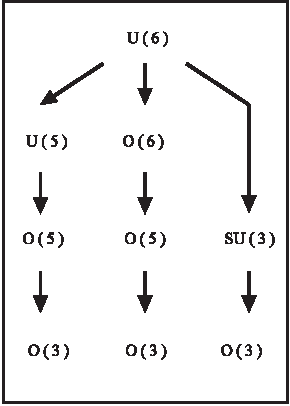
\includegraphics[scale=.65]{figure}
%
% If not, use
%\picplace{5cm}{2cm} % Give the correct figure height and width in cm
%
\caption{If the width of the figure is less than 7.8 cm use the \texttt{sidecapion} command to flush the caption on the left side of the page. If the figure is positioned at the top of the page, align the sidecaption with the top of the figure -- to achieve this you simply need to use the optional argument \texttt{[t]} with the \texttt{sidecaption} command}
\label{fig:1}       % Give a unique label
\end{figure}


\paragraph{Paragraph Heading} %
Instead of simply listing headings of different levels we recommend to let every heading be followed by at least a short passage of text. Furtheron please use the \LaTeX\ automatism for all your cross-references and citations as has already been described in Sect.~\ref{sec:2}.

Please note that the first line of text that follows a heading is not indented, whereas the first lines of all subsequent paragraphs are.

For typesetting numbered lists we recommend to use the \verb|enumerate| environment -- it will automatically render Springer's preferred layout.

\begin{enumerate}
\item{Livelihood and survival mobility are oftentimes coutcomes of uneven socioeconomic development.}
\begin{enumerate}
\item{Livelihood and survival mobility are oftentimes coutcomes of uneven socioeconomic development.}
\item{Livelihood and survival mobility are oftentimes coutcomes of uneven socioeconomic development.}
\end{enumerate}
\item{Livelihood and survival mobility are oftentimes coutcomes of uneven socioeconomic development.}
\end{enumerate}


\subparagraph{Subparagraph Heading} In order to avoid simply listing headings of different levels we recommend to let every heading be followed by at least a short passage of text. Use the \LaTeX\ automatism for all your cross-references and citations as has already been described in Sect.~\ref{sec:2}, see also Fig.~\ref{fig:2}.

Please note that the first line of text that follows a heading is not indented, whereas the first lines of all subsequent paragraphs are.

For unnumbered list we recommend to use the \verb|itemize| environment -- it will automatically render Springer's preferred layout.

\begin{itemize}
\item{Livelihood and survival mobility are oftentimes coutcomes of uneven socioeconomic development, cf. Table~\ref{tab:1}.}
\begin{itemize}
\item{Livelihood and survival mobility are oftentimes coutcomes of uneven socioeconomic development.}
\item{Livelihood and survival mobility are oftentimes coutcomes of uneven socioeconomic development.}
\end{itemize}
\item{Livelihood and survival mobility are oftentimes coutcomes of uneven socioeconomic development.}
\end{itemize}

\begin{figure}[t]
\sidecaption[t]
% Use the relevant command for your figure-insertion program
% to insert the figure file.
% For example, with the option graphics use
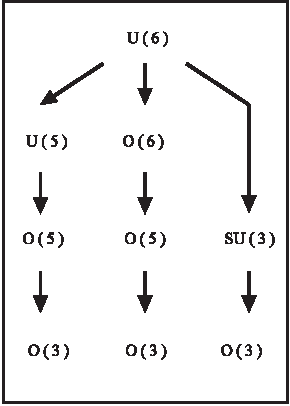
\includegraphics[scale=.65]{figure}
%
% If not, use
%\picplace{5cm}{2cm} % Give the correct figure height and width in cm
%
\caption{Please write your figure caption here}
\label{fig:2}       % Give a unique label
\end{figure}

\runinhead{Run-in Heading Boldface Version} Use the \LaTeX\ automatism for all your cross-references and citations as has already been described in Sect.~\ref{sec:2}.

\subruninhead{Run-in Heading Boldface and Italic Version} Use the \LaTeX\ automatism for all your cross-refer\-ences and citations as has already been described in Sect.~\ref{sec:2}\index{paragraph}.

\subsubruninhead{Run-in Heading Displayed Version} Use the \LaTeX\ automatism for all your cross-refer\-ences and citations as has already been described in Sect.~\ref{sec:2}\index{paragraph}.
% Use the \index{} command to code your index words
%
% For tables use
%
\begin{table}[!t]
\caption{Please write your table caption here}
\label{tab:1}       % Give a unique label
%
% For LaTeX tables use
%
\begin{tabular}{p{2cm}p{2.4cm}p{2cm}p{4.9cm}}
\hline\noalign{\smallskip}
Classes & Subclass & Length & Action Mechanism  \\
\noalign{\smallskip}\svhline\noalign{\smallskip}
Translation & mRNA$^a$  & 22 (19--25) & Translation repression, mRNA cleavage\\
Translation & mRNA cleavage & 21 & mRNA cleavage\\
Translation & mRNA  & 21--22 & mRNA cleavage\\
Translation & mRNA  & 24--26 & Histone and DNA Modification\\
\noalign{\smallskip}\hline\noalign{\smallskip}
\end{tabular}
$^a$ Table foot note (with superscript)
\end{table}
%
\section{Section Heading}
\label{sec:3}
% Always give a unique label
% and use \ref{<label>} for cross-references
% and \cite{<label>} for bibliographic references
% use \sectionmark{}
% to alter or adjust the section heading in the running head
Instead of simply listing headings of different levels we recommend to let every heading be followed by at least a short passage of text. Furtheron please use the \LaTeX\ automatism for all your cross-references and citations as has already been described in Sect.~\ref{sec:2}.

Please note that the first line of text that follows a heading is not indented, whereas the first lines of all subsequent paragraphs are.

If you want to list definitions or the like we recommend to use the Springer-enhanced \verb|description| environment -- it will automatically render Springer's preferred layout.

\begin{description}[Type 1]
\item[Type 1]{That addresses central themes pertainng to migration, health, and disease. In Sect.~\ref{sec:1}, Wilson discusses the role of human migration in infectious disease distributions and patterns.}
\item[Type 2]{That addresses central themes pertainng to migration, health, and disease. In Sect.~\ref{subsec:2}, Wilson discusses the role of human migration in infectious disease distributions and patterns.}
\end{description}

\subsection{Subsection Heading} %
In order to avoid simply listing headings of different levels we recommend to let every heading be followed by at least a short passage of text. Use the \LaTeX\ automatism for all your cross-references and citations citations as has already been described in Sect.~\ref{sec:2}.

Please note that the first line of text that follows a heading is not indented, whereas the first lines of all subsequent paragraphs are.

\begin{svgraybox}
If you want to emphasize complete paragraphs of texts we recommend to use the newly defined Springer class option \verb|graybox| and the newly defined environment \verb|svgraybox|. This will produce a 15 percent screened box 'behind' your text.

If you want to emphasize complete paragraphs of texts we recommend to use the newly defined Springer class option and environment \verb|svgraybox|. This will produce a 15 percent screened box 'behind' your text.
\end{svgraybox}


\subsubsection{Subsubsection Heading}
Instead of simply listing headings of different levels we recommend to let every heading be followed by at least a short passage of text. Furtheron please use the \LaTeX\ automatism for all your cross-references and citations as has already been described in Sect.~\ref{sec:2}.

Please note that the first line of text that follows a heading is not indented, whereas the first lines of all subsequent paragraphs are.

\begin{theorem}
Theorem text goes here.
\end{theorem}
%
% or
%
\begin{definition}
Definition text goes here.
\end{definition}

\begin{proof}
%\smartqed
Proof text goes here.
%\qed
\end{proof}

\paragraph{Paragraph Heading} %
Instead of simply listing headings of different levels we recommend to let every heading be followed by at least a short passage of text. Furtheron please use the \LaTeX\ automatism for all your cross-references and citations as has already been described in Sect.~\ref{sec:2}.

Note that the first line of text that follows a heading is not indented, whereas the first lines of all subsequent paragraphs are.
%
% For built-in environments use
%
\begin{theorem}
Theorem text goes here.
\end{theorem}
%
\begin{definition}
Definition text goes here.
\end{definition}
%
\begin{proof}
%\smartqed
Proof text goes here.
%\qed
\end{proof}
%
%
\begin{trailer}{Trailer Head}
If you want to emphasize complete paragraphs of texts in an \verb|Trailer Head| we recommend to
use  \begin{verbatim}\begin{trailer}{Trailer Head}
...
\end{trailer}\end{verbatim}
\end{trailer}
%
\begin{question}{Questions}
If you want to emphasize complete paragraphs of texts in an \verb|Questions| we recommend to
use  \begin{verbatim}\begin{question}{Questions}
...
\end{question}\end{verbatim}
\end{question}
%
%
\begin{important}{Important}
If you want to emphasize complete paragraphs of texts in an \verb|Important| we recommend to
use  \begin{verbatim}\begin{important}{Important}
...
\end{important}\end{verbatim}
\end{important}
%
\clearpage
\begin{warning}{Attention}
If you want to emphasize complete paragraphs of texts in an \verb|Attention| we recommend to
use  \begin{verbatim}\begin{warning}{Attention}
...
\end{warning}\end{verbatim}
\end{warning}

\begin{programcode}{Program Code}
If you want to emphasize complete paragraphs of texts in an \verb|Program Code| we recommend to
use

\verb|\begin{programcode}{Program Code}|

\verb|\begin{verbatim}...\end{verbatim}|

\verb|\end{programcode}|

\end{programcode}
%
\begin{tips}{Tips}
If you want to emphasize complete paragraphs of texts in an \verb|Tips| we recommend to
use  \begin{verbatim}\begin{tips}{Tips}
...
\end{tips}\end{verbatim}
\end{tips}
%
%
\begin{overview}{Overview}
If you want to emphasize complete paragraphs of texts in an \verb|Overview| we recommend to
use  \begin{verbatim}\begin{overview}{Overview}
...
\end{overview}\end{verbatim}
\end{overview}
\clearpage
\begin{backgroundinformation}{Background Information}
If you want to emphasize complete paragraphs of texts in an \verb|Background|
\verb|Information| we recommend to
use

\verb|\begin{backgroundinformation}{Background Information}|

\verb|...|

\verb|\end{backgroundinformation}|
\end{backgroundinformation}
\begin{legaltext}{Legal Text}
If you want to emphasize complete paragraphs of texts in an \verb|Legal Text| we recommend to
use  \begin{verbatim}\begin{legaltext}{Legal Text}
...
\end{legaltext}\end{verbatim}
\end{legaltext}
%
\begin{acknowledgement}
If you want to include acknowledgments of assistance and the like at the end of an individual chapter please use the \verb|acknowledgement| environment -- it will automatically render Springer's preferred layout.
\end{acknowledgement}
%
\section*{Appendix}
\addcontentsline{toc}{section}{Appendix}
%
When placed at the end of a chapter or contribution (as opposed to at the end of the book), the numbering of tables, figures, and equations in the appendix section continues on from that in the main text. Hence please \textit{do not} use the \verb|appendix| command when writing an appendix at the end of your chapter or contribution. If there is only one the appendix is designated ``Appendix'', or ``Appendix 1'', or ``Appendix 2'', etc. if there is more than one.

\begin{equation}
a \times b = c
\end{equation}
% Problems or Exercises should be sorted chapterwise
\section*{Problems}
\addcontentsline{toc}{section}{Problems}
%
% Use the following environment.
% Don't forget to label each problem;
% the label is needed for the solutions' environment
\begin{prob}
\label{prob1}
A given problem or Excercise is described here. The
problem is described here. The problem is described here.
\end{prob}

\begin{prob}
\label{prob2}
\textbf{Problem Heading}\\
(a) The first part of the problem is described here.\\
(b) The second part of the problem is described here.
\end{prob}

%%%%%%%%%%%%%%%%%%%%%%%% referenc.tex %%%%%%%%%%%%%%%%%%%%%%%%%%%%%%
% sample references
% %
% Use this file as a template for your own input.
%
%%%%%%%%%%%%%%%%%%%%%%%% Springer-Verlag %%%%%%%%%%%%%%%%%%%%%%%%%%
%
% BibTeX users please use
% \bibliographystyle{}
% \bibliography{}
%
\biblstarthook{In view of the parallel print and (chapter-wise) online publication of your book at \url{www.springerlink.com} it has been decided that -- as a genreral rule --  references should be sorted chapter-wise and placed at the end of the individual chapters. However, upon agreement with your contact at Springer you may list your references in a single seperate chapter at the end of your book. Deactivate the class option \texttt{sectrefs} and the \texttt{thebibliography} environment will be put out as a chapter of its own.\\\indent
References may be \textit{cited} in the text either by number (preferred) or by author/year.\footnote{Make sure that all references from the list are cited in the text. Those not cited should be moved to a separate \textit{Further Reading} section or chapter.} If the citatiion in the text is numbered, the reference list should be arranged in ascending order. If the citation in the text is author/year, the reference list should be \textit{sorted} alphabetically and if there are several works by the same author, the following order should be used:
\begin{enumerate}
\item all works by the author alone, ordered chronologically by year of publication
\item all works by the author with a coauthor, ordered alphabetically by coauthor
\item all works by the author with several coauthors, ordered chronologically by year of publication.
\end{enumerate}
The \textit{styling} of references\footnote{Always use the standard abbreviation of a journal's name according to the ISSN \textit{List of Title Word Abbreviations}, see \url{http://www.issn.org/en/node/344}} depends on the subject of your book:
\begin{itemize}
\item The \textit{two} recommended styles for references in books on \textit{mathematical, physical, statistical and computer sciences} are depicted in ~\cite{science-contrib, science-online, science-mono, science-journal, science-DOI} and ~\cite{phys-online, phys-mono, phys-journal, phys-DOI, phys-contrib}.
\item Examples of the most commonly used reference style in books on \textit{Psychology, Social Sciences} are~\cite{psysoc-mono, psysoc-online,psysoc-journal, psysoc-contrib, psysoc-DOI}.
\item Examples for references in books on \textit{Humanities, Linguistics, Philosophy} are~\cite{humlinphil-journal, humlinphil-contrib, humlinphil-mono, humlinphil-online, humlinphil-DOI}.
\item Examples of the basic Springer style used in publications on a wide range of subjects such as \textit{Computer Science, Economics, Engineering, Geosciences, Life Sciences, Medicine, Biomedicine} are ~\cite{basic-contrib, basic-online, basic-journal, basic-DOI, basic-mono}. 
\end{itemize}
}

\begin{thebibliography}{99.}%
% and use \bibitem to create references.
%
% Use the following syntax and markup for your references if 
% the subject of your book is from the field 
% "Mathematics, Physics, Statistics, Computer Science"
%
% Contribution 
\bibitem{science-contrib} Broy, M.: Software engineering --- from auxiliary to key technologies. In: Broy, M., Dener, E. (eds.) Software Pioneers, pp. 10-13. Springer, Heidelberg (2002)
%
% Online Document
\bibitem{science-online} Dod, J.: Effective substances. In: The Dictionary of Substances and Their Effects. Royal Society of Chemistry (1999) Available via DIALOG. \\
\url{http://www.rsc.org/dose/title of subordinate document. Cited 15 Jan 1999}
%
% Monograph
\bibitem{science-mono} Geddes, K.O., Czapor, S.R., Labahn, G.: Algorithms for Computer Algebra. Kluwer, Boston (1992) 
%
% Journal article
\bibitem{science-journal} Hamburger, C.: Quasimonotonicity, regularity and duality for nonlinear systems of partial differential equations. Ann. Mat. Pura. Appl. \textbf{169}, 321--354 (1995)
%
% Journal article by DOI
\bibitem{science-DOI} Slifka, M.K., Whitton, J.L.: Clinical implications of dysregulated cytokine production. J. Mol. Med. (2000) doi: 10.1007/s001090000086 
%
\bigskip

% Use the following (APS) syntax and markup for your references if 
% the subject of your book is from the field 
% "Mathematics, Physics, Statistics, Computer Science"
%
% Online Document
\bibitem{phys-online} J. Dod, in \textit{The Dictionary of Substances and Their Effects}, Royal Society of Chemistry. (Available via DIALOG, 1999), 
\url{http://www.rsc.org/dose/title of subordinate document. Cited 15 Jan 1999}
%
% Monograph
\bibitem{phys-mono} H. Ibach, H. L\"uth, \textit{Solid-State Physics}, 2nd edn. (Springer, New York, 1996), pp. 45-56 
%
% Journal article
\bibitem{phys-journal} S. Preuss, A. Demchuk Jr., M. Stuke, Appl. Phys. A \textbf{61}
%
% Journal article by DOI
\bibitem{phys-DOI} M.K. Slifka, J.L. Whitton, J. Mol. Med., doi: 10.1007/s001090000086
%
% Contribution 
\bibitem{phys-contrib} S.E. Smith, in \textit{Neuromuscular Junction}, ed. by E. Zaimis. Handbook of Experimental Pharmacology, vol 42 (Springer, Heidelberg, 1976), p. 593
%
\bigskip
%
% Use the following syntax and markup for your references if 
% the subject of your book is from the field 
% "Psychology, Social Sciences"
%
%
% Monograph
\bibitem{psysoc-mono} Calfee, R.~C., \& Valencia, R.~R. (1991). \textit{APA guide to preparing manuscripts for journal publication.} Washington, DC: American Psychological Association.
%
% Online Document
\bibitem{psysoc-online} Dod, J. (1999). Effective substances. In: The dictionary of substances and their effects. Royal Society of Chemistry. Available via DIALOG. \\
\url{http://www.rsc.org/dose/Effective substances.} Cited 15 Jan 1999.
%
% Journal article
\bibitem{psysoc-journal} Harris, M., Karper, E., Stacks, G., Hoffman, D., DeNiro, R., Cruz, P., et al. (2001). Writing labs and the Hollywood connection. \textit{J Film} Writing, 44(3), 213--245.
%
% Contribution 
\bibitem{psysoc-contrib} O'Neil, J.~M., \& Egan, J. (1992). Men's and women's gender role journeys: Metaphor for healing, transition, and transformation. In B.~R. Wainrig (Ed.), \textit{Gender issues across the life cycle} (pp. 107--123). New York: Springer.
%
% Journal article by DOI
\bibitem{psysoc-DOI}Kreger, M., Brindis, C.D., Manuel, D.M., Sassoubre, L. (2007). Lessons learned in systems change initiatives: benchmarks and indicators. \textit{American Journal of Community Psychology}, doi: 10.1007/s10464-007-9108-14.
%
%
% Use the following syntax and markup for your references if 
% the subject of your book is from the field 
% "Humanities, Linguistics, Philosophy"
%
\bigskip
%
% Journal article
\bibitem{humlinphil-journal} Alber John, Daniel C. O'Connell, and Sabine Kowal. 2002. Personal perspective in TV interviews. \textit{Pragmatics} 12:257--271
%
% Contribution 
\bibitem{humlinphil-contrib} Cameron, Deborah. 1997. Theoretical debates in feminist linguistics: Questions of sex and gender. In \textit{Gender and discourse}, ed. Ruth Wodak, 99--119. London: Sage Publications.
%
% Monograph
\bibitem{humlinphil-mono} Cameron, Deborah. 1985. \textit{Feminism and linguistic theory.} New York: St. Martin's Press.
%
% Online Document
\bibitem{humlinphil-online} Dod, Jake. 1999. Effective substances. In: The dictionary of substances and their effects. Royal Society of Chemistry. Available via DIALOG. \\
http://www.rsc.org/dose/title of subordinate document. Cited 15 Jan 1999
%
% Journal article by DOI
\bibitem{humlinphil-DOI} Suleiman, Camelia, Daniel C. O'Connell, and Sabine Kowal. 2002. `If you and I, if we, in this later day, lose that sacred fire...': Perspective in political interviews. \textit{Journal of Psycholinguistic Research}. doi: 10.1023/A:1015592129296.
%
%
%
\bigskip
%
%
% Use the following syntax and markup for your references if 
% the subject of your book is from the field 
% "Computer Science, Economics, Engineering, Geosciences, Life Sciences"
%
%
% Contribution 
\bibitem{basic-contrib} Brown B, Aaron M (2001) The politics of nature. In: Smith J (ed) The rise of modern genomics, 3rd edn. Wiley, New York 
%
% Online Document
\bibitem{basic-online} Dod J (1999) Effective Substances. In: The dictionary of substances and their effects. Royal Society of Chemistry. Available via DIALOG. \\
\url{http://www.rsc.org/dose/title of subordinate document. Cited 15 Jan 1999}
%
% Journal article by DOI
\bibitem{basic-DOI} Slifka MK, Whitton JL (2000) Clinical implications of dysregulated cytokine production. J Mol Med, doi: 10.1007/s001090000086
%
% Journal article
\bibitem{basic-journal} Smith J, Jones M Jr, Houghton L et al (1999) Future of health insurance. N Engl J Med 965:325--329
%
% Monograph
\bibitem{basic-mono} South J, Blass B (2001) The future of modern genomics. Blackwell, London 
%
\end{thebibliography}


%\chapter{Reactive Systems}

\section{Reactive Manifesto}

Organizations working in disparate domains are independently discovering patterns for building software that look the same. These systems are more robust, more resilient, more flexible and better positioned to meet modern demands.

These changes are happening because application requirements have changed dramatically in recent years. Only a few years ago a large application had tens of servers, seconds of response time, hours of offline maintenance and gigabytes of data. Today applications are deployed on everything from mobile devices to a cloud-based clusters running thousands of multi-core processors. Users expect milliseconds response times and 100\% up-time. Data is measured in petabytes. Today's demands are simply not met by yesterday's software architecture.

A coherent approach to systems architecture is needed, and all necessary aspects are already recognized individually. Systems must be (Figure \ref{fig:responsive}):
\begin{itemize}
    \item Responsive;
    \item Resilient;
    \item Elastic;
    \item Message-Driven.
\end{itemize}
Systems that have all of the above characteristics are called Reactive Systems. They are more:
\begin{itemize}
    \item Flexible;
    \item Loosely-coupled;
    \item Scalable.
\end{itemize}
Because of that these ones are easier to develop and amenable to change. They are significantly more tolerant of failure and when failure does occur they meet it with elegance rather than disaster.  

\begin{figure}[ht]
\caption{Characteristics of a Reactive Systems}
\centering
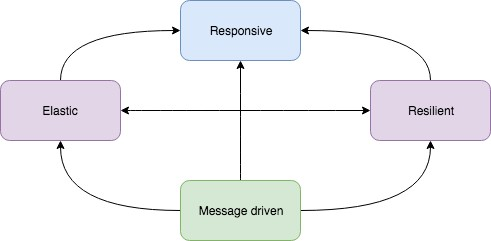
\includegraphics[width=1\textwidth]{reactive}
 \label{fig:responsive}
\end{figure}

\paragraph{Responsive}
The system responds in a timely manner if at all possible. Responsiveness means that problems may be detected quickly and deal with it effectively. 
Characteristics:
\begin{itemize}
    \item Cornerstone of usability;
    \item Systems must respond in a fast and consistent fashion if at all possible;
    \item Responsive systems build user confidence.
\end{itemize}

\paragraph{Resilient}
The system stays responsive in the face of failure. This applies not only highly-available, mission-critical systems -- any system that is not resilient will be unresponsive after a failure. Attributes:
\begin{itemize}
    \item Provides responsiveness, despite failures;
    \item Achieved through replication, isolation, containment, delegation;
    \item Failure are isolated to a single component;
    \item Recovery is delegated to an external component (If you're the failing component, then you're not reliable enough to handle your own failure. If the system goes down it can't restart itself. So an external component is needed to monitor it and restart if necessary.). 
\end{itemize}

\paragraph{Elastic}
The system stays responsive under varying workload. Reactive Systems can react to changes in the input rate by increasing or decreasing the resources allocated to service these inputs. 

\begin{itemize}
    \item Provides responsiveness, despite increase/decrease in load;
    \item Implies zero contention and no central bottlenecks. (As a directive because it's impossible in a real scenario);
    \item Predictive auto scaling techniques can be used to support elasticity;
    \item Scaling up provides responsiveness during peak, while scaling down improving cost effectiveness. 
\end{itemize}

\paragraph{Message Driven}
Reactive Systems rely on asynchronous message-passing to establish a boundary between components that ensures loose coupling, isolation and location transparency. This boundary also provides the means to delegate failure as messages.
\begin{itemize}
    \item Responsiveness, Resilience and Elasticity are all supported by a Message Driven architecture;
    \item Messages are asynchronous and non-blocking;
    \item Provides Loose coupling, isolation, location transparency;
    \item Resources are consumed only while active, meaning you don't have a situation where you make a request and that request is blocking, and you're stuck waiting for a response from someone who could take a long time getting back, or not respond back at all. While you're waiting, you're consuming any number of physical resources, threads, CPU cycles etc;
    \item Send message and release the resource. Response will then come back asynchronously.
\end{itemize}

Employing explicit message-passing enables load-management, elasticity, and flow control by shaping and monitoring the message queues in the system applying back-pressure when necessary. Location transparent messaging as a means of communication makes it possible for the management of failure to work with the same constructs and semantics across a cluster or within single host. Non-blocking communication allows recipients to only consume resources while active, leading to less system overhead.

\subsection{Goals}
The main goals to use Reactive Systems are:
\begin{itemize}
    \item Scales from 10 to 10 million users;
    \item Consumes only the resources necessary to support the current load;
    \item Handles failures with little to no effect on the user;
    \item Can be distributed across tens, hundreds, or even thousands of machines;
    \item Maintains a consistent level of quality and responsiveness despite failures.
\end{itemize}

\section{Reactive Systems vs Reactive Programming}
Reactive systems can be implemented using reactive programming or not. Reactive Systems are related to an architectural style that allows multiple individual applications to coalesce as a single unit, reacting to its surroundings, while remaining aware of each other. 

Reactive Programming is a subset of asynchronous programming and a paradigm where the availability of new information drives the logic forward rather than having control flow driven by a thread-of-execution.

\begin{itemize}
    \item Reactive Programming can be used to support the construction of Reactive Systems;
    \item It supports breaking problems into small, discrete steps that are executed in an asynchronous/non-blocking fashion, usually via a callback mechanism (Futures/Promises, Streams, RxJava, RxScala);
    \item A system that uses Reactive Programming is not necessarily a Reactive System (You could build a system with reactive programming techniques and then deployed onto a single node. It's not a reactive system because if this node crashes, the whole system will be down).
\end{itemize}

\section{Actor Model}
The actor model is a conceptual model to deal with concurrent computation. It defines some general rules for how system's components should behave and interact with each other. Characteristics:
\begin{itemize}
    \item Programming paradigm that supports the construction of Reactive Systems;
    \item Just because you use the Actor Model, doesn't mean that you've built a Reactive System;
    \item It's Message Driven, all communication is asynchronous and non-blocking;
    \item Provides abstractions that give us Elasticity and Resilience;
    \item It can therefore be used to build Responsive software;
    \item On the JVM, the Actor Model is implemented with Akka\footnote{It's what we are using to produce reactive applications. There is other solutions. As an alternative you can take a look at \href{http://scalecube.io/}{scalecube}.}.
    \item All computation occurs inside of Actors;
    \item Each actor has an address;
    \item Actors communicate only through asynchronous messages.
\end{itemize}

\subsection{Location Transparency}

\begin{figure}[ht]
\caption{Actor model location transparency}
\centering
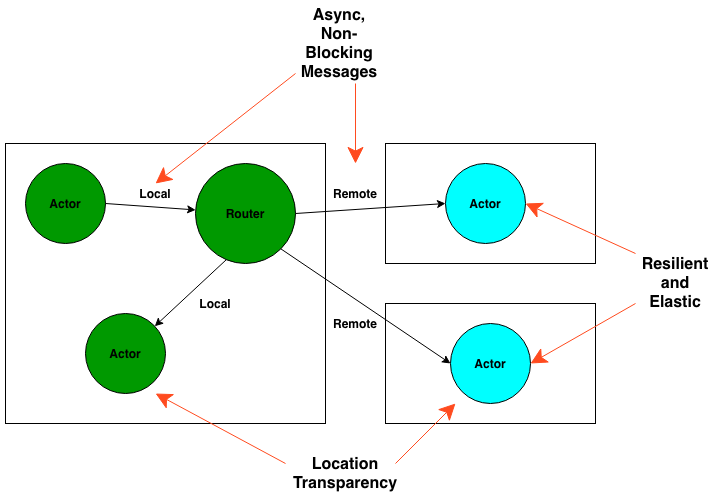
\includegraphics[width=1\textwidth]{location_transparency}
 \label{fig:location_transparency}
\end{figure}

Everything in Akka is designed to work in a distributed setting: all interactions of actors use purely message passing and everything is asynchronous. The key for enabling this is go to from remote to local by way of optimization instead of trying go from local to remote by way generalization. In summary:
\begin{itemize}
    \item Message Driven nature of Actors supports Location Transparency (Figure~\ref{fig:location_transparency});
    \item Actors communicate using the same technique, regardless of location;
    \item Local vs Remote is mostly configuration (Configure that a particular router can route to these routees. Communication mechanisms don't change at all). Original actor sends message with no knowledge of location of where that message is going to;
    \item No specific technique of API to send to a remote actor. API is identical for Remote and Local;
    \item Location transparency enables actors to be Resilient and Elastic (Resilient because we can deploy actors across multiple nodes and elastic because if we have high load, we can add more routees on more pieces of hardware, or remove to scale down.).
\end{itemize}

You can find more information about Remote vs Local transparency in the Table~\ref{tab:loctransparency}

\begin{table}[ht]
  \begin{center}
    \caption{Location transparency vs Transparent Remoting}
    \label{tab:loctransparency}
    \begin{tabularx}{\textwidth}{|Y|Y|} \hline 
      \textbf{Location Transparency} & \textbf{Transparent Remoting}\\\hline\hline
       Remote calls look like local calls. & Local calls look like remote calls.\\\hline
       Hides the fact that you're making remote calls. & Assumes you're always doing remote calls.\\\hline
       Hides potential failure scenarios (E.g. Network failures). For example, because it will look like a local call, you might not think to deal with that possibility. & You have to assume remote failure scenarios can occur (E.g. Network failures).\\\hline
    \end{tabularx}
  \end{center}
\end{table}

\paragraph{Importance of the Actor Model}
There are other reactive tools but most of them only support part of the Reactive Principles. So to achieve that you need to combine different technologies to build a Reactive System. Generally if you build a Reactive System without Actors you will probably need:
\begin{itemize}
    \item Service Registry;
    \item Load Balancer;
    \item Message Bus.
\end{itemize}

In contrast with the Actor Model can be reactive at the level of actors. So if you build you system based on actors and micro services this should be enough.
The actor model facilitates the the design of Reactive design because:
\begin{itemize}
    \item It's Message Driven by default;
    \item It's location transparent providing Elasticity and Resilience through distribution;
    \item It's Responsive because of the previous two points; (Take a look at the Figure~\ref{fig:responsive}). 
\end{itemize}

\section{References}

\begin{thebibliography}{9}

\bibitem{reactive_manifesto} 
\href{https://www.reactivemanifesto.org/}{\textit{Reactive Manifesto}}, 2014.

\bibitem{reactive_arch_1} 
Wade Waldron, 
\href{https://academy.lightbend.com/courses/course-v1:lightbend+LRA-IntroToReactive+v1/about}{\textit{Reactive Architecture(1): Introduction to Reactive Systems}}, Lightbend 2020.

\bibitem{reactive_prog_sys} 
Jonas Bon\'er and Viktor Klang,
\href{https://www.lightbend.com/blog/white-paper-understanding-reactive-programming-vs-reactive-systems}{\textit{Reactive Programming versus Reactive Systems}}, Lighbend 2020.

\bibitem{reactive_explained}
Grace Jansen and Peter Gollmar,
\href{https://www.ibm.com/downloads/cas/YEEQBXND}{\textit{Reactive Systems Explained: Jump-Start Your Journey to Reactive Architecture}}, 
IBM 2020
\end{thebibliography}

\chapter{Domain Driven Design}

Domain-Driven design (DDD) is the concept that the structure and language of your code (class names, class methods, class variables) should match the business domain. DDD objective is to ease the creation of complex applications by connecting the related pieces of the software into an evolving model. Generally DDD is the architectural approach that is used to design large system. The guidelines used by DDD are highly compatible with those reactive architecture so as a result you'll often see them used together.

\section{Domain}

A domain is a sphere of knowledge. In the context of software, it refers to the business idea that we are modeling. A domain is defined by the Domain-Experts that understand the business idea, but not necessarily the software. The key goal of DDD is to build a model that the domain experts can understand. So we can conclude:
\begin{itemize}
    \item The model represents our understanding of the domain;
    \item The software is an implementation of the model.
\end{itemize}

\section{Ubiquitous Language}

Ubiquitous Language is the term by Eric Evans in order to build a language shared by the team, developers, domain experts, and other participants.
Regardless of how software is designed, it will need to reflect a clear and modeled Ubiquitous Language within a Delimited Context. Ubiquitous Language (UL) has the following characteristics:
\begin{itemize}
    \item Must be expressed in the Domain Model:
    \begin{itemize}
        \item Terminology in the UL comes from the domain experts;
        \item Words originate in the domain and are used in the software;
        \item Avoid taking software terms and introducing them into the domain;
        \item Domain Experts and Developers should be able to have a conversation without resorting to software terms. 
    \end{itemize}
    \item Unites the people of the project team;
    \item Eliminates inaccuracies and contradictions from domain experts;
    \item Not a business language imposed by domain experts or a language used in industries;
    \item Evolves over time, it is not define entirely in a single meeting;
    \item Concepts that are not part of the Ubiquitous Language should be rejected.
\end{itemize}

\section{Subdomains}

We can say that Domain is a scope where one works and how one works, in the other words, it refers to the space of the problem for which we are acting, its entities, behaviors and rules. It is from the Domain that we design our Domain Models, which solutions that seek to meet the needs of the domain. It is a mistake that we can create a single Domain Model. If you try to do that it will surely fail. 
We can see a restaurant domain in the Figure~\ref{fig:domain} as example.

\begin{itemize}
    \item Business Domains are often large and complicated;
    \item They contain many ideas, actions and rules that interact in complex ways;
    \item Trying to model a large domain can become problematic;
    \item Therefore, we separate our large domains into subdomains.
\end{itemize}

\begin{figure}[ht]
\caption{Example of a Restaurant Domain}
\centering
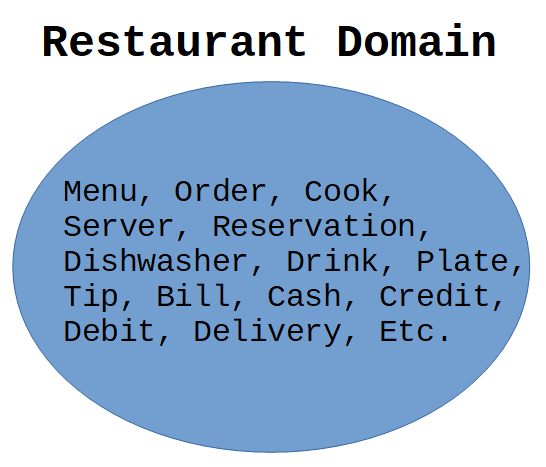
\includegraphics[width=.5\textwidth]{domain}
 \label{fig:domain}
\end{figure}

DDD requires the decomposition of the Domain into Subdomains, which facilitates our understanding. Subdomains are created by grouping related ideas, actions and rules. Some concepts may exist in multiple subdomains but they \emph{may not be the same}. In the Restaurant's Domain lets look at the \emph{Customer} concept:
\begin{itemize}
    \item Shared concepts (Customer) may not be identical initially;
    \item They may also look identical initially but them evolve differently over time. So we should avoid abstraction of the concept;
    \item Customer in the Reservation Subdomain (Figure~\ref{fig:subdomain}) may have details that are important in other part of the business.
\end{itemize}

Each Subdomain ends up having its own Ubiquitous Language and Model. The language and model for a subdomain is called a \emph{Bounded Context}.

\begin{figure}[ht]
\caption{Example of a Restaurant Reservation Subdomain}
\centering
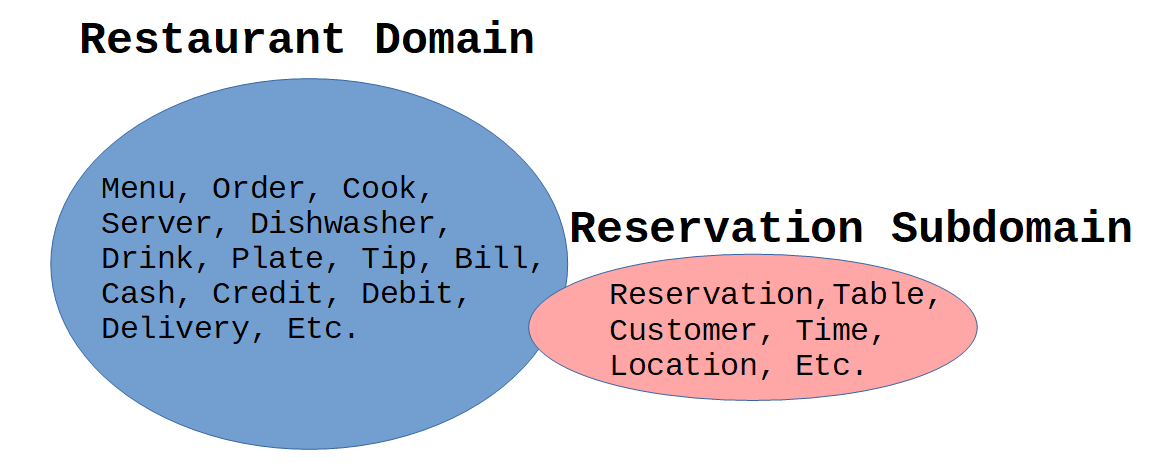
\includegraphics[width=1\textwidth]{subdomain}
 \label{fig:subdomain}
\end{figure}

\section{Bounded Contexts}

A Bounded Context is a logical boundary of a domain where particular terms and rules apply consistently. Inside this boundary, all terms, definitions, and concepts form the Ubiquitous Language. Taking the Restaurant Example we can define the following bounded context:
\begin{itemize}
    \item A customer in the Reservations Context will probably need to include certain details, eg phone number;
    \item Might not need to know the address, but in the Deliveries Context the address must be required;
    \item The model for a Customer in Reservations would likely not be the same as a model of a customer in other parts of the business;
    \item \emph{Bounded Context} is the combination of the \emph{Model} and the \emph{Ubiquitous Language};
    \item Subdomains and Bounded Contexts usually map in a kind of 1 to 1 relationship;
    \item Subdomains or Bounded Context are good starting points for building Reactive Microservices;
    \item Generally don't want all our bounded contexts built into a single service\footnote{With this approach you are building a monolith.}. 
\end{itemize}

\paragraph{Understanding Bounded Contexts}

From one Bounded Context to the meaning of a concept may change dramatically.
\begin{itemize}
    \item In a restaurant when talking to a server, an \emph{Order} has a very specific meaning. The client is the Customer;
    \item When speaking to the person who manages inventory for the restaurant \emph{Order} means something completely different. Restaurant is the Customer.
\end{itemize}

We also need to observe how the details of the model change.
\begin{itemize}
    \item In a restaurant, when the kithen is preparing an Order they don't care about prices;
    \item When a customer pays for the Order, price is critical;
    \item It is the same Order but the relevant details of that Order change;
    \item Depending in what part of the business, we are working in, the details of an Order will change.
\end{itemize}

\paragraph{Guidelines to determine Bounded Contexts}

\begin{itemize}
    \item Consider human interaction. Different areas of the domain that are handled by different groups of people, suggests a natural division. Might imply separate Bounded Context;
    \item Look for change in the Ubiquitous Language. If the use of language or the meaning of that language changes, that may suggest a new context (The Order that the server takes versus the Order for inventory.);
    \item Look for varying or unnecessary information (EmployeeId is very important in an Employee but meaningless in a Customer.);
    \item Strongly separated Bounded Contexts will result in smooth workflows. An awkward workflow may signal a misunderstanding of the domain, or that you've broken up your Domain / Bounded Context incorrectly;
    \item If a Bounded Context has too many dependencies it may be overcomplicated, you may have drawn the separation lines (subdomains) incorrectly.
\end{itemize}

You can find a real example of a Bounded Context in the Figure~\ref{fig:bounded}

\begin{figure}[ht]
\caption{Real division of a Domain}
\centering
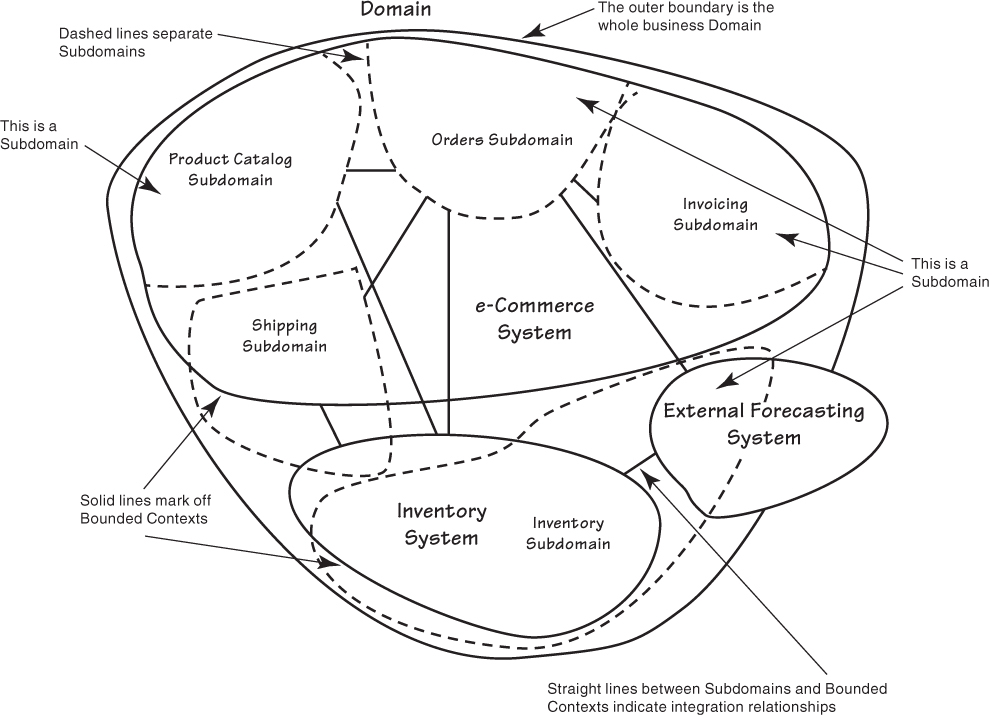
\includegraphics[width=1\textwidth]{bounded}
 \label{fig:bounded}
\end{figure}

\section{Strategies to Define the DDD Model}

\subsection{Event First Domain Driven Design}

Traditionally, DDD focused on the objects within the Domain. In more recent times, the techniques have evolved a bit and now we have \emph{Event First DDD} or \emph{Event Storming}. Event First DDD places the focus on the activities or events that occur in the domain. Eg.
\begin{itemize}
    \item Customer makes a reservation;
    \item Server places an order;
    \item Food is served to the customer.
\end{itemize}

Using Event First DDD, we start by defining the activities, then group those activities to find logical system boundaries.

\paragraph{Subject--Verb--Object Notation}
Subject--Verb--Object Notation provide us a consistent way to phrase our activities or events in the domain.
The sentences are composed by the subject first, the object as last and the verb in the middle. Example:

\begin{quote}
    Host checks current reservation.
\end{quote}
\begin{description}
    \item[Subject] Host;
    \item[Object] Reservation;
    \item[Verb] Check.
\end{description}

Note that \emph{current} is just a simple modifier on the object.

\paragraph{Direct versus Indirect Objects}

Lets look at the following sentence:
\begin{quote}
    Bartender collects Payment for a Drink Order.
\end{quote}

So, is \emph{Payment} or \emph{Order} the Object? 
In this context:
\begin{itemize}
    \item Payment is the Direct Object;
    \item Drink Order is the Indirect Object.
\end{itemize}

So they are \emph{both} Objects. We're less concerned with direct and indirect but we need to be aware that there will be often be more than one object. 

\subsection{Event Storming}

Event Storming is a workshop format for quickly exploring complex business domains. It is:
\begin{description}
    \item[Powerful] Allow many practitioners to come up with a comprehensive model of a complete business flow in hours instead weeks;
    \item[Engaging] The whole idea is to bring people with the questions and people who know the answer in the same room and to build a model together;
    \item[Efficient] The resulting model is perfectly align with the DDD model (particularly Event Sourcing) and allows for a quick determination of Context and Aggregate boundaries;
    \item[Easy] The notation is ultra-simple. No complex UML that cut off participants from the heart of the discussion.
    \item[Fun] People are energized and deliver more than they expected.
\end{description}

You can find more about event storm information in the Section \ref{chp2references} in the \cite{wiksto20} and \cite{albbra13} items.

\begin{figure}[ht]
\caption{Event Storming Layout}
\centering
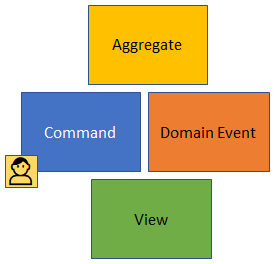
\includegraphics[width=.5\textwidth]{storming.png}
 \label{fig:storming}
\end{figure}

\section{Anti-Corruption Layers}
Anti-Corruption Layers (ACL) is a pattern that implements a fa\c cade or adapter layer between different subsystems that don't share the same semantics. 
This pattern is exemplified on the Figure~\ref{fig:aclfull}. So the goal of using ACLs is keep the clarity and purity between our Bounded Contexts. It's important to recognize that:
\begin{itemize}
    \item Each Bounded Contexts may have domain concepts that are unique. In the Figure~\ref{fig:acl}, we have the reservations context and our customer context. There are certain aspects of a Customer that are unique to the Customer Context. There are certain aspects of a customer that are unique to the customer, they don't matter to the reservation (eg. Address);
    \item Concepts are not always compatible from one context to the next. Sometimes, what happens is that you end up with a concept that is called one thing in the reservations context and called another thing in the customer context, or may end up with a situation where something is not compatible in such a way that it requires a translation of some kind (different units for example);
    \item Anti-Corruption Layers introduced to translate these concepts;
    \item ACL will prevent Bounded Contexts from leaking into each other: 
    \begin{itemize}
        \item Don't want to just come up with an abstraction or some way to make it the same across all Bounded Contexts;
        \item This would create coupling, that we need to avoid. Would need to make updates everywhere across all contexts, for minor changes in one.
    \end{itemize}
    \item ACLs help the Bounded Context to stand alone. It looks at whatever that Customer Context representation is and it translates it into a representation that is unique to the reservation service. Strips out unnecessary info like address in this case. This therefore maintains purity in the Reservation Context. This prevents leakage between Bounded Contexts;
    \item Standing alone. If we have a caching layer inside of the ACL, in case of failure, the service can be able to operate.
\end{itemize}

To implement the Anti-Corruption Layer we commonly use an Abstract Interface.
\begin{itemize}
    \item Interface represents the pure domain representation of the data;
    \item Implementation of the interface does the necessary translation.
\end{itemize}

\begin{figure}[ht]
\caption{Anti-Corruption Layer}
\centering
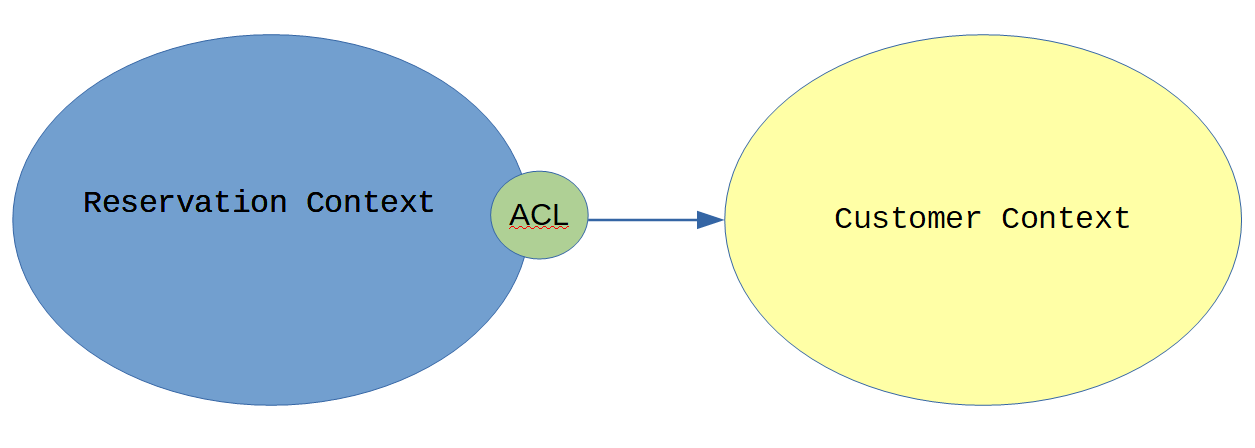
\includegraphics[width=1\textwidth]{acl}
 \label{fig:acl}
\end{figure}


\begin{figure}[ht]
\caption{Anti-Corruption Layer Example}
\centering
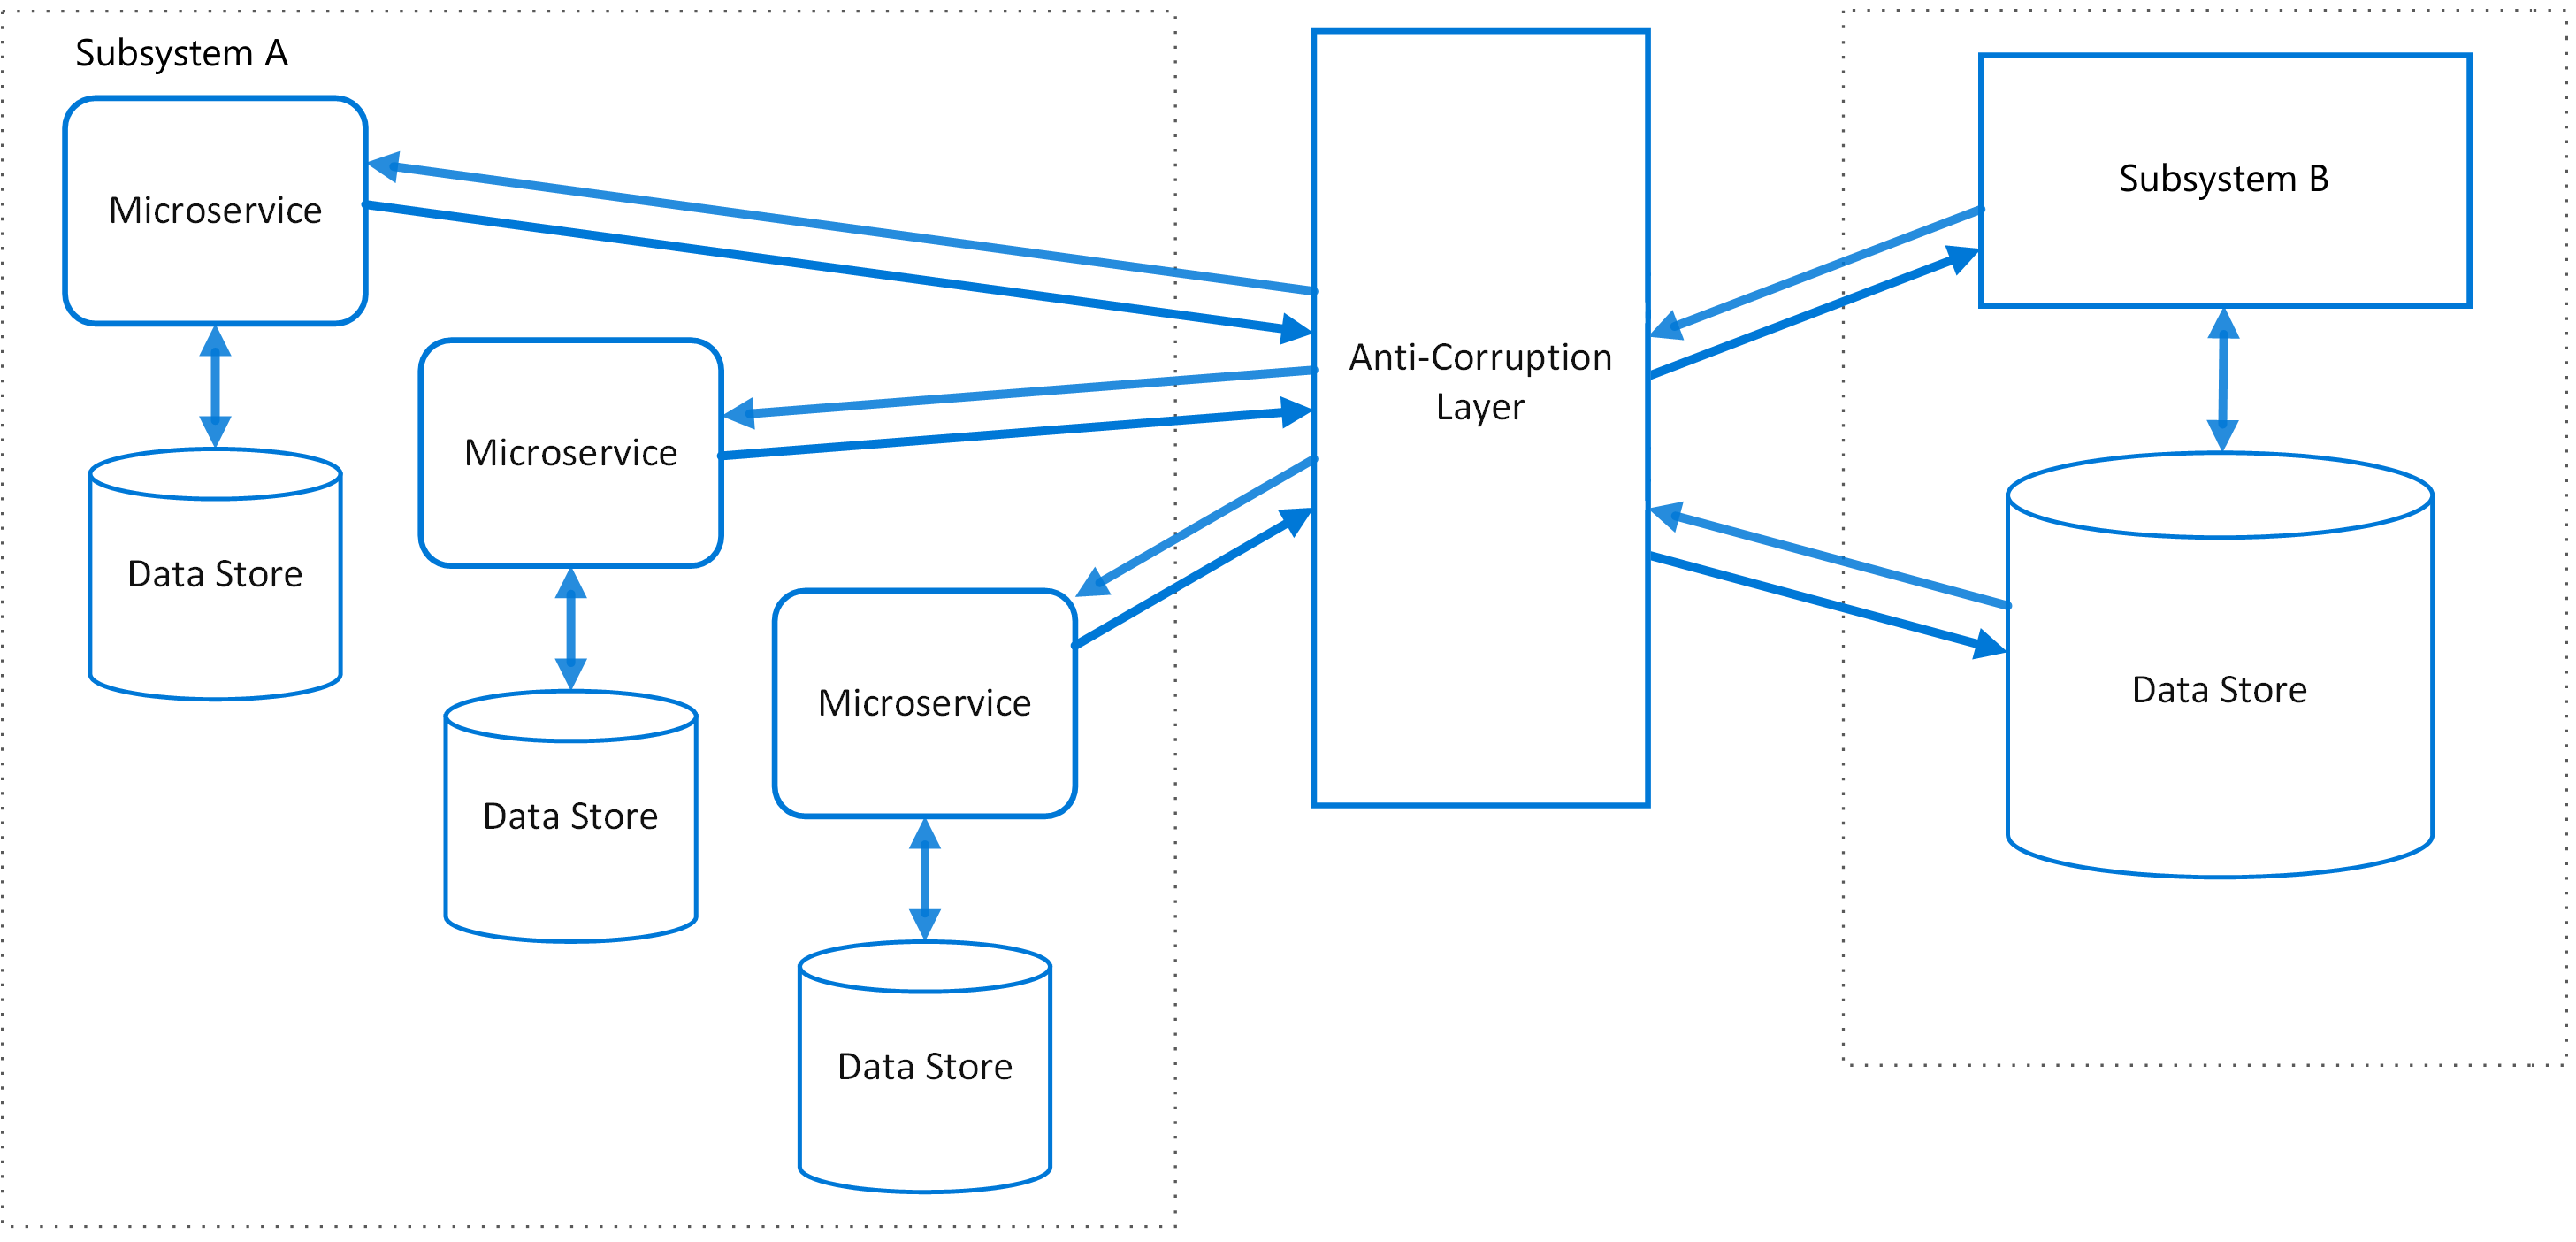
\includegraphics[width=1\textwidth]{anti-corruption-layer}
 \label{fig:aclfull}
\end{figure}

\subsection{Anti-Corruption Layer for Legacy Systems}

Organizations often choose to integrate legacy systems with their replacements, either for the short term or indefinitely. But there's a risk: connecting the old to the new can drag unwanted problems into what is a clean design. Legacy systems suffer from outdated protocols, data models, schemas and/or obsolete APIs. To interface legacy systems, new(er) pipeline applications may need to support legacy features that don't align with modern architectural techniques. Based in the example in the Figure~\ref{fig:acllegacy}, ACLs can help with:
\begin{itemize}
    \item In this case, the domain may be messy or unclear, ACL has the job of keeping the mess of that legacy system out of our pure Bounded Context;
    \item Keeps our Bounded Context pure;
    \item Prevents our domain from having to deal with the mess;
    \item ACL may be implemented in the Legacy System, or in the Bounded Context, or Both as the example provided;
    \item It's recommended that every time a pure microservice or a Pure Bounded Context has to communicate with another external service of some kind, it should do throught an ACL;
    \item With the legacy service, because of the complexity of it, may want to expose an API that's just for the Reservations Context which then has a bit cleaner that what the messy legacy system would typically be exposing.
\end{itemize}

\begin{figure}[ht]
\caption{Anti-Corruption Layer for Legacy Systems}
\centering
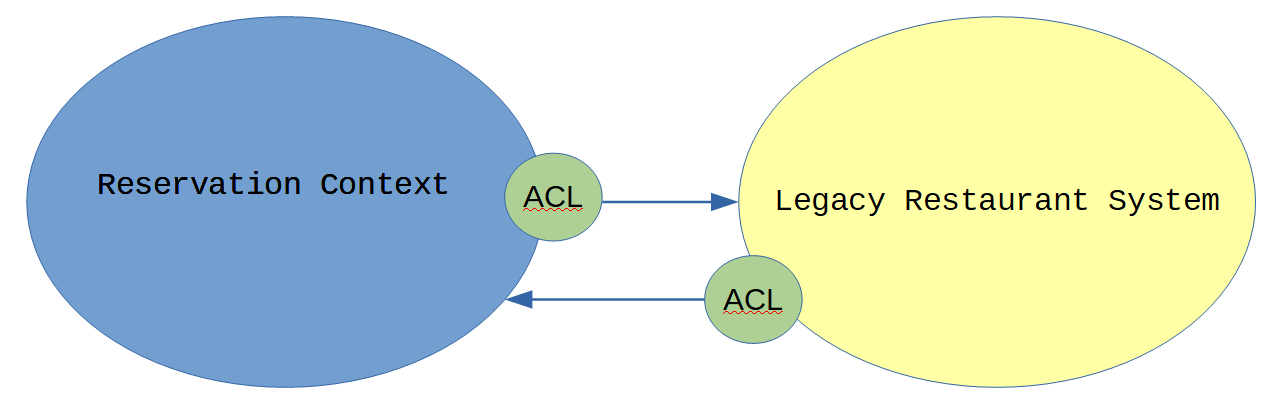
\includegraphics[width=1\textwidth]{acl_legacy}
 \label{fig:acllegacy}
\end{figure}

\section{Context Maps}

\section{Domain Activities}

\subsection{Commands}

\subsection{Events}

\subsection{Queries}

\section{Domain Objects}

\subsection{Values}

\subsection{Entities}

\subsection{Aggregates}

\section{Domain Abstractions}

\subsection{Services}

\subsection{Factories}

\subsection{Repositories}

\section{Hexagonal Architecture}

\section{References} \label{chp2references}

\begin{thebibliography}{9}

\bibitem{wiksto20}
Wikipedia,
\href{https://en.wikipedia.org/wiki/Event_storming}{\textit{Event Storming}}, 
2020

\bibitem{albbra13}
Alberto Brandolini,
\href{http://ziobrando.blogspot.com/2013/11/introducing-event-storming.html}{\textit{Introducing Event Storming}}, 
2013

\end{thebibliography}

%\chapter{Microservices}
%\chapter{Consistency}
%\chapter{Messaging}
%\chapter{CQRS \& ES}
%%%%%%%%%%%%%%%%%%%%%% appendix.tex %%%%%%%%%%%%%%%%%%%%%%%%%%%%%%%%%
%
% sample appendix
%
% Use this file as a template for your own input.
%
%%%%%%%%%%%%%%%%%%%%%%%% Springer-Verlag %%%%%%%%%%%%%%%%%%%%%%%%%%

\appendix
\motto{All's well that ends well}
\chapter{Chapter Heading}
\label{introA} % Always give a unique label
% use \chaptermark{}
% to alter or adjust the chapter heading in the running head

Use the template \emph{appendix.tex} together with the Springer document class SVMono (monograph-type books) or SVMult (edited books) to style appendix of your book.


\section{Section Heading}
\label{sec:A1}
% Always give a unique label
% and use \ref{<label>} for cross-references
% and \cite{<label>} for bibliographic references
% use \sectionmark{}
% to alter or adjust the section heading in the running head
Instead of simply listing headings of different levels we recommend to let every heading be followed by at least a short passage of text. Furtheron please use the \LaTeX\ automatism for all your cross-references and citations.


\subsection{Subsection Heading}
\label{sec:A2}
Instead of simply listing headings of different levels we recommend to let every heading be followed by at least a short passage of text. Furtheron please use the \LaTeX\ automatism for all your cross-references and citations as has already been described in Sect.~\ref{sec:A1}.

For multiline equations we recommend to use the \verb|eqnarray| environment.
\begin{eqnarray}
\vec{a}\times\vec{b}=\vec{c} \nonumber\\
\vec{a}\times\vec{b}=\vec{c}
\label{eq:A01}
\end{eqnarray}

\subsubsection{Subsubsection Heading}
Instead of simply listing headings of different levels we recommend to let every heading be followed by at least a short passage of text. Furtheron please use the \LaTeX\ automatism for all your cross-references and citations as has already been described in Sect.~\ref{sec:A2}.

Please note that the first line of text that follows a heading is not indented, whereas the first lines of all subsequent paragraphs are.

% For figures use
%
\begin{figure}[t]
\sidecaption[t]
%\centering
% Use the relevant command for your figure-insertion program
% to insert the figure file.
% For example, with the option graphics use
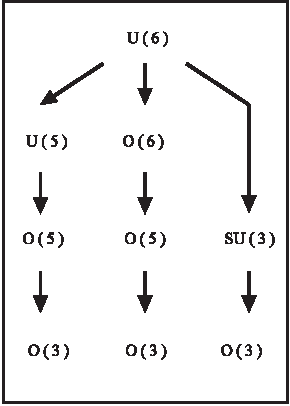
\includegraphics[scale=.65]{figure}
%
% If not, use
%\picplace{5cm}{2cm} % Give the correct figure height and width in cm
%
\caption{Please write your figure caption here}
\label{fig:A1}       % Give a unique label
\end{figure}

% For tables use
%
\begin{table}
\caption{Please write your table caption here}
\label{tab:A1}       % Give a unique label
%
% For LaTeX tables use
%
\begin{tabular}{p{2cm}p{2.4cm}p{2cm}p{4.9cm}}
\hline\noalign{\smallskip}
Classes & Subclass & Length & Action Mechanism  \\
\noalign{\smallskip}\hline\noalign{\smallskip}
Translation & mRNA$^a$  & 22 (19--25) & Translation repression, mRNA cleavage\\
Translation & mRNA cleavage & 21 & mRNA cleavage\\
Translation & mRNA  & 21--22 & mRNA cleavage\\
Translation & mRNA  & 24--26 & Histone and DNA Modification\\
\noalign{\smallskip}\hline\noalign{\smallskip}
\end{tabular}
$^a$ Table foot note (with superscript)
\end{table}
%


%\backmatter
%%%%%%%%%%%%%%%%%%%%%%%acronym.tex%%%%%%%%%%%%%%%%%%%%%%%%%%%%%%%%%%%%%%%%%
% sample list of acronyms
%
% Use this file as a template for your own input.
%
%%%%%%%%%%%%%%%%%%%%%%%% Springer %%%%%%%%%%%%%%%%%%%%%%%%%%

\Extrachap{Glossary}


Use the template \emph{glossary.tex} together with the Springer document class SVMono (monograph-type books) or SVMult (edited books) to style your glossary\index{glossary} in the Springer layout.


\runinhead{glossary term} Write here the description of the glossary term. Write here the description of the glossary term. Write here the description of the glossary term.

\runinhead{glossary term} Write here the description of the glossary term. Write here the description of the glossary term. Write here the description of the glossary term.

\runinhead{glossary term} Write here the description of the glossary term. Write here the description of the glossary term. Write here the description of the glossary term.

\runinhead{glossary term} Write here the description of the glossary term. Write here the description of the glossary term. Write here the description of the glossary term.

\runinhead{glossary term} Write here the description of the glossary term. Write here the description of the glossary term. Write here the description of the glossary term.
%
\Extrachap{Solutions}

\section*{Problems of Chapter~\ref{intro}}

\begin{sol}{prob1}
The solution\index{problems}\index{solutions} is revealed here.
\end{sol}


\begin{sol}{prob2}
\textbf{Problem Heading}\\
(a) The solution of first part is revealed here.\\
(b) The solution of second part is revealed here.
\end{sol}


%\printindex

\end{document}





